
\chapter{EVALUACIJA PIV TOČNOSTI}
\label{chap:Poglavlje_4}
Kvaliteta točnosti PIV mjerenja određena je veličinom greške unutar samih mjerenja. Sveukupna greška mjerenja prilikom PIV analize je kombinacija širokog spektra aspekata koji idu od postavki samog setup-a mjerenja, snimanja pa sve do metoda evaluacije. Na \textit{Slici \ref{sl:4.1}} prikazani su neki od glavnih parametara koje je potrebno uzeti u obzir prilikom PIV mjerenja.
\begin{figure}[h]  
	\centering
	%\usepackage{graphicx}
	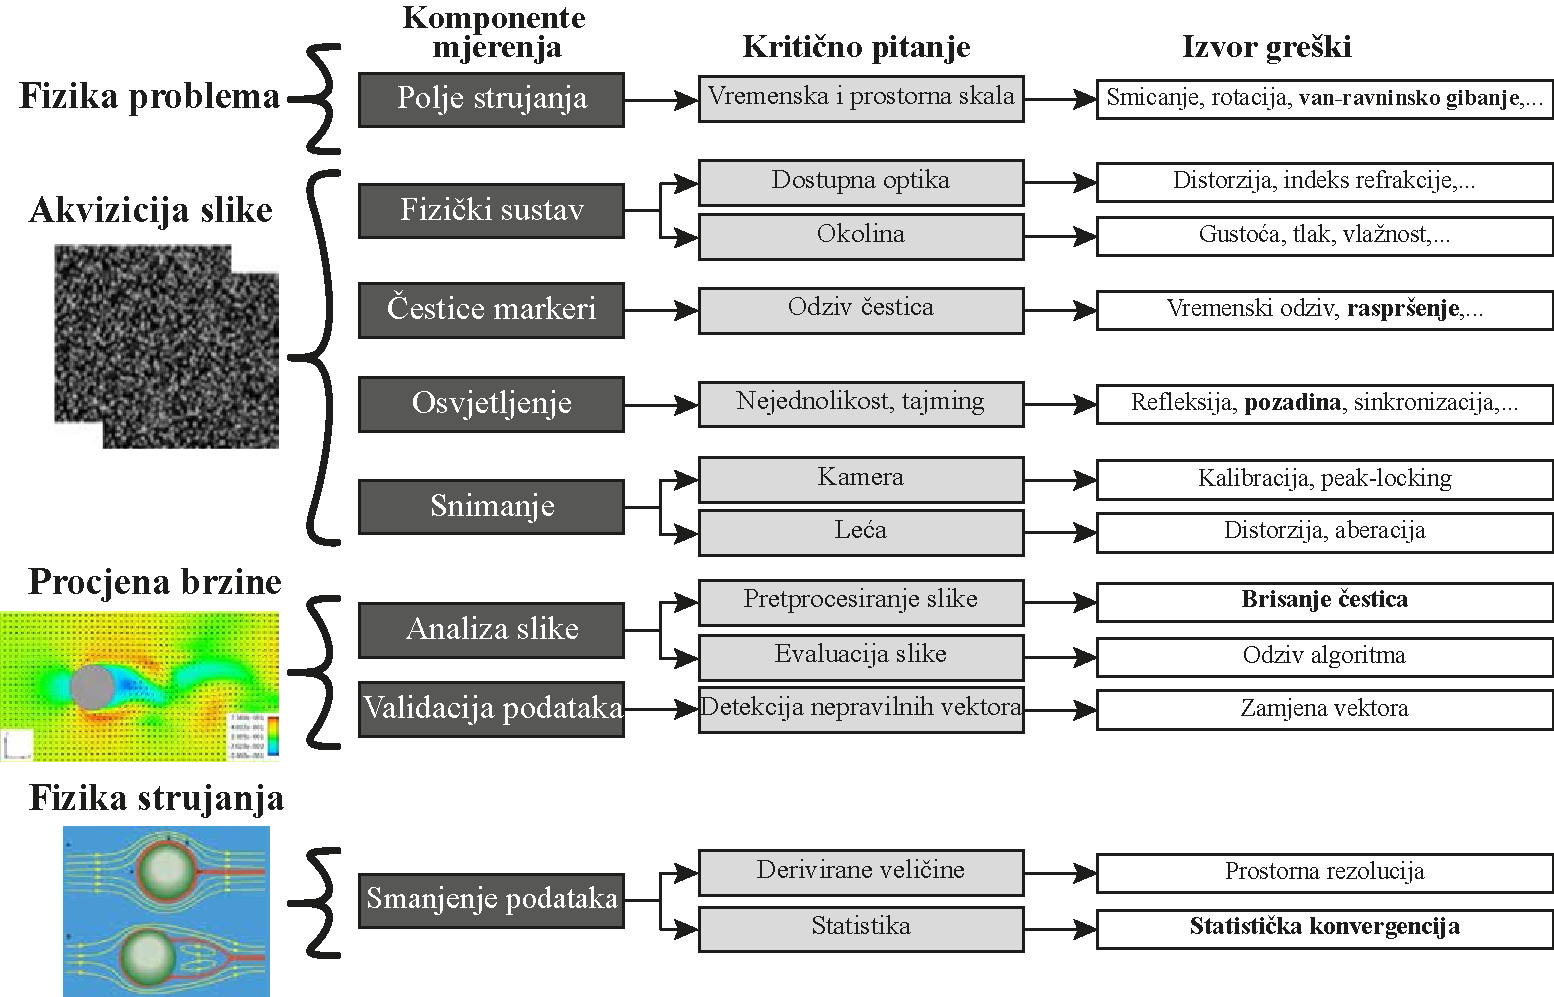
\includegraphics[width=16cm]{./4_PIVNesigurnost/slika4_1.pdf} 
	\caption{Kvantifikacija glavnih komponenti PIV mjerenja, te nekih od najvažnijih izvora pogrešaka (podebljane su greške koje se smatraju jako slučajne) \cite{sciacchitano2019_article}}
	\label{sl:4.1}
\end{figure}
\par
U DPIV analizi postoje dva glavna izvora nesigurnosti u mjerenjima: pristrana pogreška $\epsilon_{pristr.}$ i slučajna pogreška $\epsilon_{slu\textup{č}.}$ koji zajedno doprinose ukupnoj greški mjerenja $\epsilon$ \cite{raffel2018_book}. Pristrana pogreška određuje istinitost procjene pomaka. Istinitost je definirana kao "preklapanje" između srednje vrijednosti (velike količine) izmjerenih podataka te stvarnog pomaka. Slučajna pogreška određuje preciznost procjene pomaka. Preciznost se definira kao mjera veličine (širine) razmaka između procijenjenih pomaka. Moguće je da su mjerenja jako precizna, ali srednja vrijednost mjerenja nije točna jer se jako razlikuje od stvarnog pomaka (\textit{Slika \ref{sl:4.2}}). Istinitost i preciznost skupa definiraju točnost mjerenja PIV sustava. 
\begin{figure}[h]  
	\centering
	%\usepackage{graphicx}
	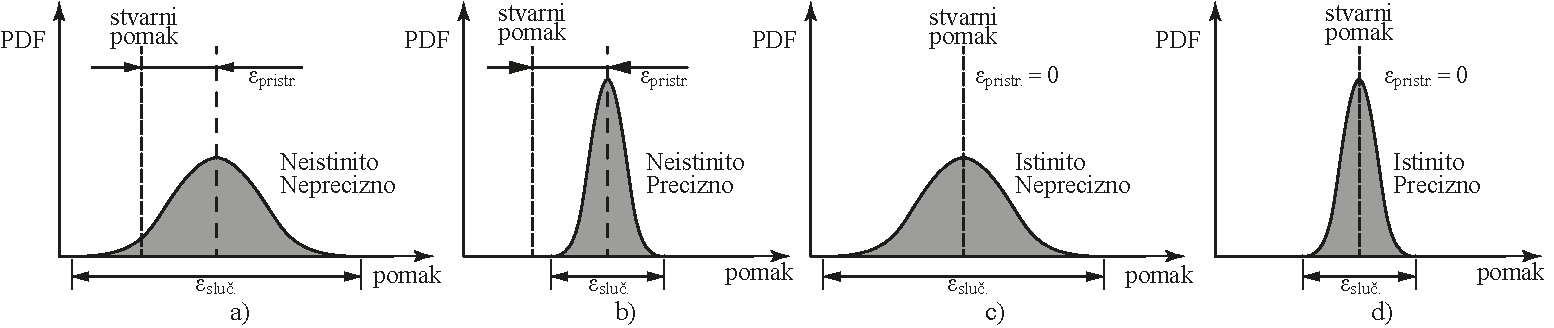
\includegraphics[width=16cm]{./4_PIVNesigurnost/slika4_2.pdf} 
	\caption{Definicija točnosti tj. istinitosti i preciznosti u PIV analizi}
	\label{sl:4.2}
\end{figure}
\par
Kod određivanja pristrane i slučajne pogreške, potreban je ogroman broj podataka i da bi rezultati bili relevantni potrebne su statističke simulacije koje upotrebljavaju veliki broj podataka (npr. Monte Carlo simulacija). Naravno, dodatno kako bi se odredila pogreška potrebno je znati i vrijednost stvarnog pomaka. Najjednostavniji način da se zadovolje ovi uvjeti je korištenje sintetičkih čestičnih slika (\textit{eng. synthetic particle images}), čija će upotreba biti kasnije objašnjena.  Pristrana pogreška računa se pomoću sljedeće formule:
\begin{equation}
	\epsilon_{pristr.}=\frac{1}{n}\sum_{i=1}^{n}x_{i} - x_{stv}
	\label{eqn:4.1}
\end{equation}
gdje $x_{i}$ predstavlja pomak izmjeren određenim DPIV algoritmom, dok je $x_{stv}$ stvarni pomak koji se generira u sintetičkoj slici.\\
Slučajna pogreška računa se putem izraza:
\begin{equation}
	\epsilon_{slu\textup{č}.}=\sqrt{\frac{1}{n}\sum_{i=1}^{n}(\overline{x}-x_{i})}
	\label{eqn:4.2}
\end{equation}
gdje $\overline{x}$ predstavlja srednju izmjerenu vrijednost pomaka, a $n$ broj čestica. Pristrana pogreška uzrokovana je tzv. peak-locking efektom koji postoji u većini kros-korelacijskih algoritama. Peak-locking (poznato i kao pristranost pixela) je ozbiljna pogreška pristranosti u PIV evaluaciji gdje izmjerene vrijednost lokacija i pomaka čestica su pristrana prema cjelobrojnim vrijednostima (integer). Do pogreške dolazi zbog "fittanja" glatke krivulje kroz diskretnu distribuciju intenziteta u korelacijskoj matrici tijekom pretraživanja korelacijskih vrhova. Pristrana pogreška je funkcija pomaka, veličina pogreške najviše ovisi o korelacijskom algoritmu, tehnici subpixelske aproksimacije, te promjeru čestice. U \textit{Tablici \ref{tab:4.1}} prikazano je testiranje nekoliko DPIV korelacijskih algoritama, te su na sljedećim slikama prikazani i rezultati točnosti testiranih algoritama uzimajući u obzir nekoliko eksperimentalnih situacija \cite{thielicke2014_phd} (sve simulacije su napravljene sa brojem čestica $n\geq 930 000$).
\begin{table}[h]
	\centering
	\caption{Testirani DPIV algoritmi (rezultati na \textit{Slikama \ref{sl:4.3} \ref{sl:4.4}, \ref{sl:4.5}}) \cite{thielicke2014_phd}}
	\resizebox{\textwidth}{!}{%
	\begin{tabular}{llllll}
		\hline
		\rowcolor[HTML]{C0C0C0} 
		\multicolumn{2}{l}{\cellcolor[HTML]{C0C0C0}\textbf{Parametar}} & \textbf{DKK}           & \textbf{DFT}           & \textbf{DFT multi-linearni} & \textbf{DFT multi-spline} \\ \hline
		\multicolumn{2}{l}{CLAHE, veličina {[}px{]}}                   & $50$                   & $50$                   & $50$                        & $50$                      \\
		\multicolumn{2}{l}{DPIV tehnika}                               & DKK                    & DFT                    & DFT                         & DFT                       \\
		\multicolumn{2}{l}{Subpixelska aproksimacija}                  & Gauss $3$-točke & Gauss $3$-točke & Gauss $3$-točke      & Gauss $3$-točke    \\
		\multicolumn{2}{l}{Deformacija prozora ispit.}                 & -                      & -                      & linearna                    & spline                    \\
		\multicolumn{2}{l}{Preklapanje {[}\%{]}}                       & $50$                   & $50$                   & $50$                        & $50$                      \\
		1. prolaz:          & Veličina proz. ispit. {[}px{]}          & $16\cdot 16$           & $16\cdot 16$           & $64\cdot 64$                & $16\cdot 16$              \\
		2. prolaz:          & Veličina proz. ispit. {[}px{]}          & -                      & -                      & $32\cdot 32$                & $16\cdot 16$              \\
		3. prolaz:          & Veličina proz. ispit. {[}px{]}          & -                      & -                      & $16\cdot 16$                & $16\cdot 16$              \\
		4. prolaz:          & Veličina proz. ispit. {[}px{]}          & -                      & -                      & -                           & $16\cdot 16$              \\ \hline
	\end{tabular}}
	\label{tab:4.1}
\end{table}
\par
Subpixelska aproksimacija također teži cjelobrojnim vrijednostima, a taj efekt postaje sve gori kada su čestice jako malene veličine. Snimke u kojima su čestice manje od 3 pixela daju jako uske vrhove u korelacijskoj matrici, što dovodi do toga da aproksimacija Gauss-ovom funkcijom se ne može izvršiti. Opisani problem može se vidjeti na \textit{Slici \ref{sl:4.3}}. Ovdje, svi testirani DPIV algoritmi imaju značajan nedostatak točnosti, zbog toga što se svi oslanjaju na  subpixelsku aproksimaciju u $3$ točke koja očito nije prikladna za snimke sa vrlo malenim česticama. Nadalje vidljiv je značajan pad vrijednosti greške za snimke sa promjerom čestice od 3 mm (\textit{Slika \ref{sl:4.4}}), te 5 mm (\textit{Slika \ref{sl:4.5}})
\begin{figure}[h]  
	\centering
	%\usepackage{graphicx}
	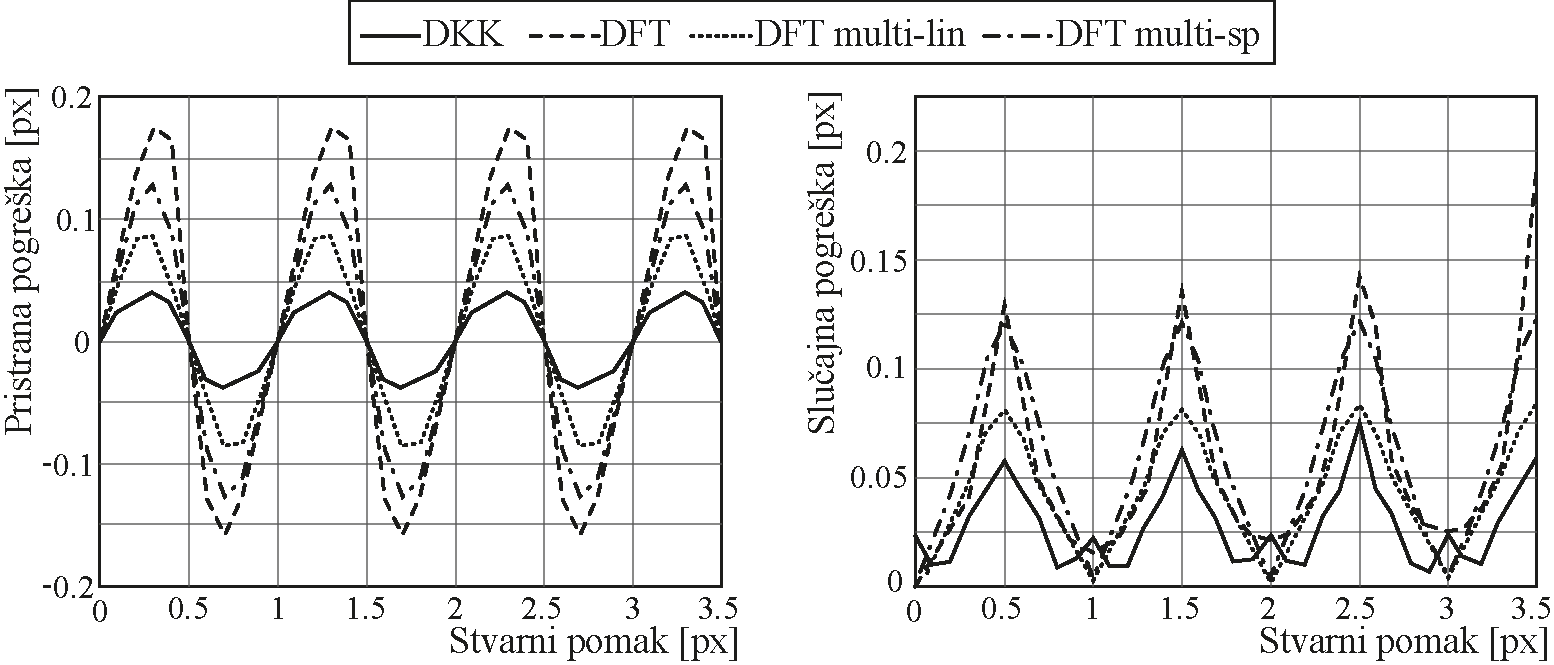
\includegraphics[width=16.5cm]{./4_PIVNesigurnost/slika4_3.pdf} 
	\caption{Pristrana i slučajna pogreška za čestice markere promjera 1 pixel}
	\label{sl:4.3}
\end{figure}
\begin{figure}[h]  
	\centering
	%\usepackage{graphicx}
	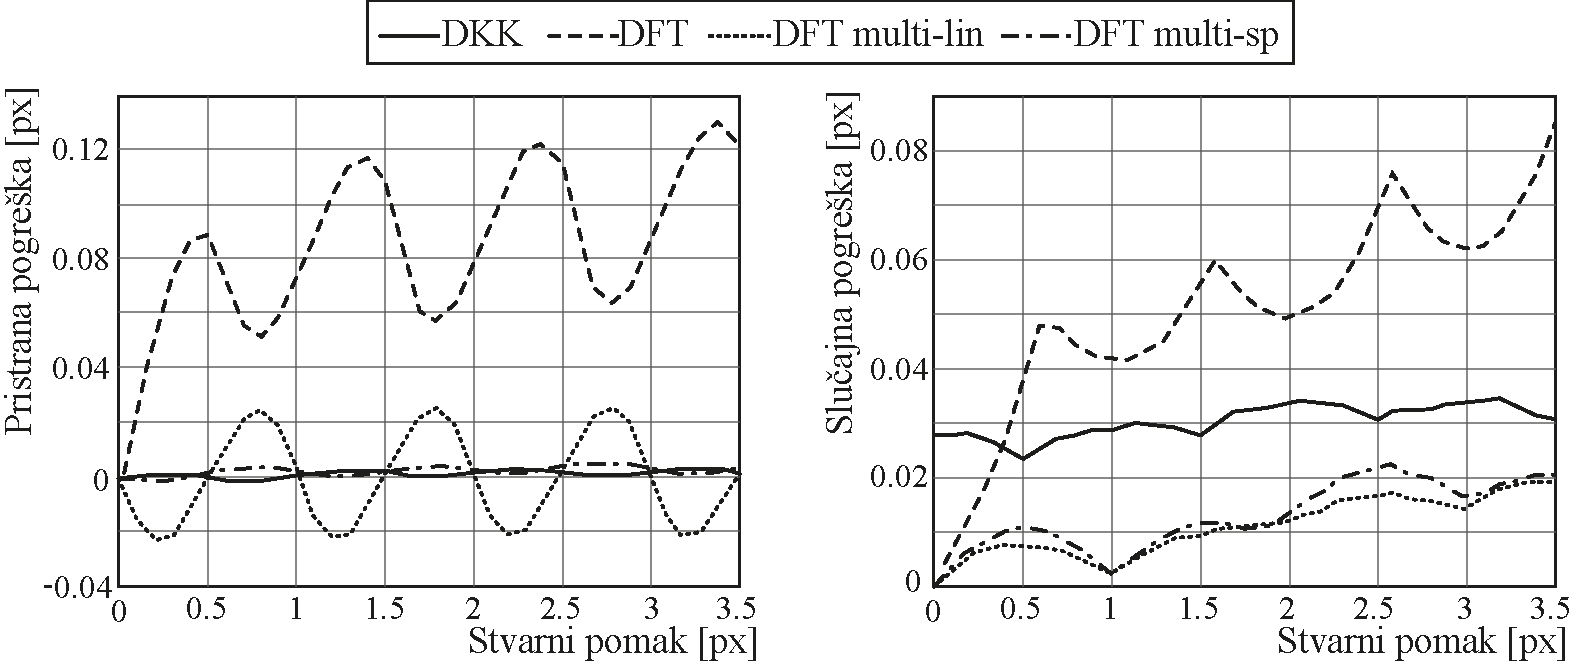
\includegraphics[width=16.5cm]{./4_PIVNesigurnost/slika4_4.pdf} 
	\caption{Pristrana i slučajna pogreška za čestice markere promjera 3 pixel-a}
	\label{sl:4.4}
\end{figure}
\begin{figure}[h]  
	\centering
	%\usepackage{graphicx}
	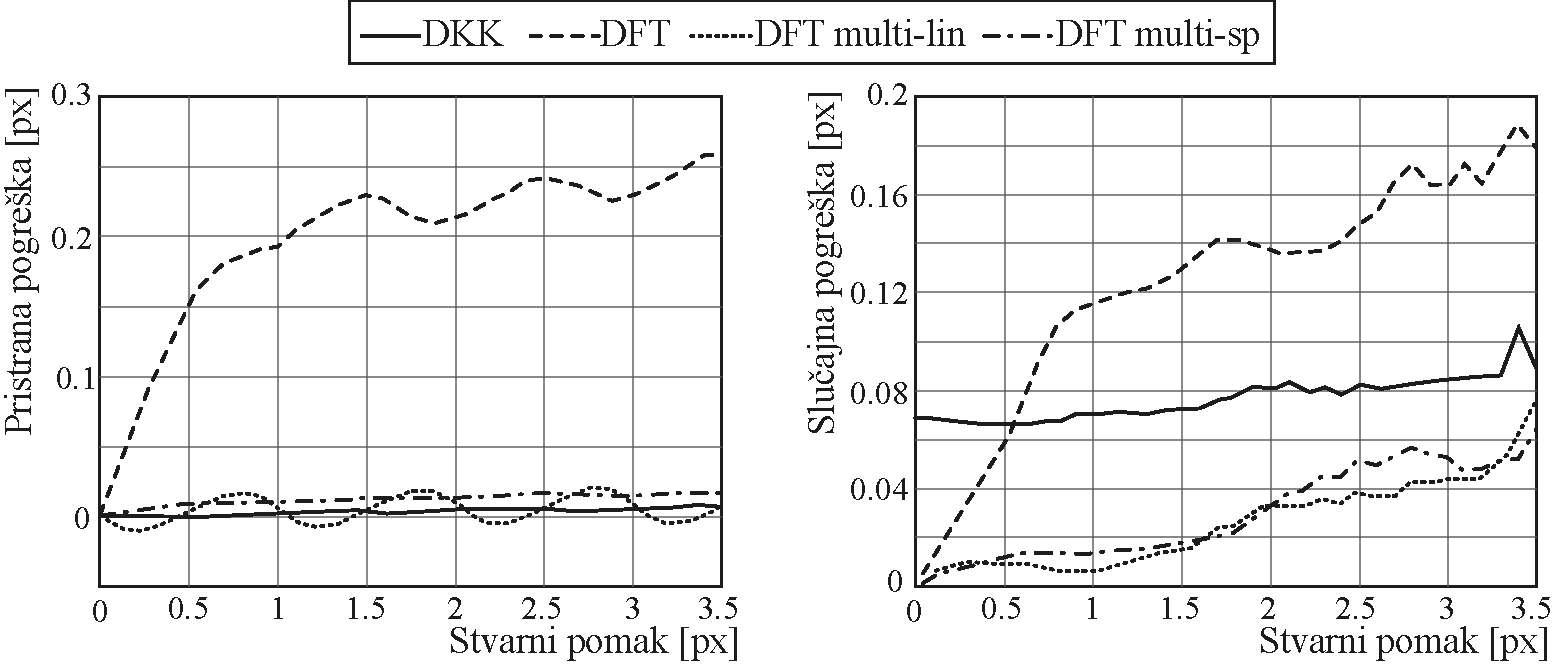
\includegraphics[width=16.5cm]{./4_PIVNesigurnost/slika4_5.pdf} 
	\caption{Pristrana i slučajna pogreška za čestice markere promjera 5 pixel-a}
	\label{sl:4.5}
\end{figure}
\FloatBarrier
\section{Dinamički raspon brzina ($DVR$) i dinamički prostorni raspon ($DSR$)}
Tipična točnost PIV mjerenja brzine je unutar 1\%, dok je prostorna rezolucija unutar 1 milimetra \cite{adrian1997dynamic}. Korisnost PIV mjerenja obično je karakterizirana sa svojom točnosti i prostornom rezolucijom. Međutim, nijedna od ovih veličina ne opisuje kompletno sposobnosti PIV sustava, te se zbog toga koriste pojmovi dinamički raspon brzine $DVR$ (\textit{eng. Dynamic Velocity Range}) i dinamički prostorni raspon $DSR$ (\textit{eng. Dynamic Spatial Range}). Dinamički raspon brzina definiran je kao omjer maksimalne brzine $U_{max}$ (koji se može mjeriti sa određenim postavkama PIV sustava) sa minimalnom razlučivosti fluktuacija mjerenih brzina $\sigma_{U}$ (srednji kvadratni korijen pogrešaka brzine), tj. jednostavnije omjerom maksimalne i minimalne razlučive brzine:
\begin{equation}
	DVR=\frac{U_{max}}{\sigma_{U}}
	\label{eqn:4.3}
\end{equation}
U svojim počecima PIV sustavi imali dosta niske vrijednosti $DVR$ (u rasponu 10-100), te zbog toga razloga mjerenja nisu mogla razlučiti određene dijelove strujanja u slučaju da je dolazilo do značajnih promjena brzine. Čak i ako nije bilo velikih varijacija brzine, nizak raspon $DVR$ dovodio je do toga de je trebalo oprezno prilagoditi parametre mjerenja da brzine strujanja upadnu u zadano područje. Dinamički prostorni raspon ili raspon skala definira se kao omjer vidnog polja čestica i najmanje razlučive prostorne varijacije, tj. može se shvatiti kao veličina koja govori o tome koliko je moguće mjerenje najmanjih skala strujanja (npr. granični sloj) uključenih unutar većih skala strujanja:
\begin{equation}
	DSR=\frac{x_{max}}{D_{I}}
	\label{eqn:4.4}
\end{equation} 
gdje je $x_{max}$ duljina senzora kamere u pixelima, a $D_{I}$ duljina prozora ispitivanja također u pixelima. Kako bi se kompenzirao gubitak informacija unutar malenih skala strujanja moguća je opcija uvećati optičko povećanje sustava snimanja $M_{0}$ ili dodatno povećati koncentraciju čestica markera u protoku. Na taj način mjerena nesigurnost može biti smanjena na račun manjeg vidnog polja strujanja, što će naravno dovesti do toga da se izgube veće skale strujanja koje su i prvotno bile od veće zanimljivosti.
\par
U današnje vrijeme, mnogo snažniji laseri, osjetljive digitalne kamere, te sofisticirane analize snimki i dobivenih vektora i brzina, uz sve bolje metode ubacivanja čestica markera dovele su do toga da PIV mjerenja budu znatno pouzdanija. Međutim i dalje ostaje veliki problem PIV mjerenja sa niskom nesigurnošću, zbog toga što je iznimno složeno podešavanje parametara sustava koji se ne mogu mijenjati individualno, zbog velike ovisnosti jednih o drugima. Prema tome i dalje je veoma važno poznavanje osnovnih znanja i mogućnosti kako PIV sustava, tako i same fizike strujanja.
\section{Generiranje sintetičkih PIV snimki}
Kako slučajna i pristrana pogreška u digitalnoj PIV evaluaciji mogu biti jedino poznate ako su točno poznati i stvarni pomaci čestica, potrebno je poznavati iznose pomaka. U početku su s koristile PIV snimke iz izrazito mirnih strujanja u kojima su sa velikom sigurnošću bile poznate veličine i karakteristike strujanja. Sa tim poznatim i određenim karakteristikama mogli su se testirati i kalibrirati određeni PIV softveri, tj. korelacijski signali koji u najvećoj mjeri doprinose mjernoj nesigurnosti. Međutim, svaki put kada bi se trebalo raditi drugačije mjerenje bilo je potrebno napraviti i nove posebne kalibracije gdje se svaki parametar mora oprezno provjeriti, što je izrazito neefikasan i spor proces. Jedan od pristupa je korištenje umjetno stvorenih (sintetičkih) PIV snimki koje bi zajedno sa numeričkom simulacijom (Monte Carlo) uspješno mogle ispitati valjanost PIV softvera. Procjena nesigurnosti bazirana na sintetičkim snimkama pruža tri glavne prednosti:
\begin{enumerate}[label=\textbf{\arabic*)}, leftmargin=*, align=left, itemsep=0em, topsep=0em]
	\item Moguća je potpuna kontrola parametara koji se koriste u simulaciji (nasuprot eksperimentima gdje postoji mnogo nesigurnosti kao što su: lokalna gustoća, temperatura, viskoznost, čestica unutar okoline, razni problemi za kamerom i osvjetljenjem).
	\item Moguća je individualna kontrola parametara, što je nemoguće postići u eksperimentima zbog međusobne ovisnosti.
	\item Raspon mijenjanja vrijednosti parametara može biti povećan ili smanjen čak i izvan granica raspona koje je eksperimentalno moguće postići.
\end{enumerate}
Glavni nedostatak ovom pristupu je u tome da ipak nije moguće simulirati sve moguće fizičke efekte koji se pojavljuju u strujanju, te simulirane snimke mogu biti prejednostavne.
\par
Sintetičke slike su generirane u PIVlab softveru po preporukama u literaturi \cite{raffel2018_book}, te čestice unutar njih moraju zadovoljiti određene karakteristike: promjer, oblik, prostornu gustoću, dubinu slike, itd.. Sve čestice imaju Gauss-ov profil intenziteta sa točno određenim promjerom koji je zadan jednadžbom (\ref{eqn:4.5}). 
\begin{equation}
	I(x, y) = I_{0} \exp\left(\frac{-(x-x_{0})^{2}-(y-y_{0})^{2}}{\frac{1}{8}d_{\tau}^{2}}\right)
	\label{eqn:4.5}
\end{equation}
gdje $x_{0}$ i $y_{0}$ predstavljaju sredinu lokacije čestice, $I_{0}$ vrijednost intenziteta u sredini čestice (najveća vrijednost), te $d_{\tau}$ promjer čestice. Faktor $I_{0}$ također je u funkciji pozicije čestice u smjeru Z-osi, kako bi se uzela u obzir debljina laserske zrake (\textit{Slika \ref{sl:4.6} lijevo}). Poznati broj čestica je slučajno postavljen, te simulirana laserska zraka također ima Gauss-ov profil intenziteta (jednadžba \ref{eqn:4.6}) kako bi se u obzir uzele 3D lokacije čestica u stvarnosti (\textit{Slika \ref{sl:4.6}}). 
\begin{equation}
	I_{0}(Z)=q\exp \left( -\frac{1}{\sqrt{2\pi}} \left|\frac{2Z^{2}}{\Delta Z_{0}^{2}}\right|^{s} \right)
	\label{eqn:4.6}
\end{equation}
gdje $q$ predstavlja efikasnost kojom čestice raspršuju obasjanu svjetlost, $\Delta Z_{0}$ predstavlja debljinu svjetlosne zrake na kojoj intenzitet opada na $-\frac{1}{\sqrt{2\pi}}\approx0.67$ maksimalnog intenziteta koji se nalazi u sredini zrake ($Z=0$), a $s$ je faktor oblika profila (za $s=2$ profil intenziteta ima oblik Gauss-ove funkcije, dok za veće vrijednosti poprima oblik tzv. top-hat funkcije kako je prikazano na \textit{Slika \ref{sl:4.6} desno}). Nadalje, pretpostavlja se da promjer čestica $d_{\tau}$ je mnogo manji od debljine laserske zrake $\Delta Z_{0}$. Generiranje sintetičke slike se vrši na način da se prvo generira slučajni broj koji specificira lokaciju čestice ($x_{0}, y_{0}, z_{0}$) unutar 3D laserske zrake (\textit{Slika \ref{sl:4.6} lijevo}). Maksimalni intenzitet $I_{0}(z_{0})$ se odredi uz pomoć jednadžbe \ref{eqn:4.6}. Nakon čega se ta vrijednost uvrsti u jednadžbu \ref{eqn:4.5} gdje se izračuna vrijednost intenziteta svijetla koju uhvati svaki pixel. Naknadno je moguće dodavanje raznih šumova koji bi još opisali dodatno uvjete prilikom stvarnog PIV mjerenja (npr. šum senzora kamere).
\begin{figure}[h]  
	\centering
	%\usepackage{graphicx}
	\includegraphics[width=13cm]{./4_PIVNesigurnost/slika4_6.jpg} 
	\caption{3D prostor laserske zrake sa generiranim sintetičkim česticama (lijevo), te funkcije kojima je moguće opisati profil intenziteta laserske svjetlosti prema jednadžbi \ref{eqn:4.5} (desno)\cite{raffel2018_book}}
	\label{sl:4.6}
\end{figure}
\par
Kako bi se generirala sljedeća slika, to jest pomak čestica, obično se koriste neka od generičkih strujanja koja se dobiju analitički (osnovana laminarna strujanja) ili numerički (turbulentno) te se na osnovi njihovih rješenja generiraju nove slike sa pomaknutim česticama.
\FloatBarrier
\section{Utjecajni parametri na korelacijski signal}
U ovom potpoglavlju ukratko će biti objašnjeni utjecaji nekih od parametra koje je moguće kontrolirati pri generiranju sintetičkih snimki, a koji značajno utječu na točnosti DPIV algoritama. Variranjem jednog po jednog od ovih parametara omogućava određivanje osjetljivosti, te samim time i optimizaciju kasnijeg eksperimentalnog postupka:
\begin{description}[style=unboxed,leftmargin=0cm]
	\item[Promjer čestica markera] Veličina čestica u PIV eksperimentima obično dosta varira, te značajno utječe na točnost analize. U literaturama \cite{guezennec1990statistical} ustanovljen je pad točnosti DPIV analize za čestice koje imaju promjer veći od 2 pixela, te je pronađen optimalni promjer od 1.5 pixela\cite{raffel2018_book}. Također jačina utjecaja promjera čestice ovisi i o korištenom DPIV algoritmu (\textit{Slika \ref{sl:4.7}}). Na slici je vidljivo kako slučajne pogreške za DKK i obični DFT algoritam imaju lokalni minimum na promjeru od 1.8-2 pixela. Dok je za DFT sa tehnikama deformacije prozora ispitivanja minimum pomaknut udesno, te se vidi kako ovi algoritmi imaju značajno manji iznos slučajne pogreške.
	\begin{figure}[H]  
		\centering
		%\usepackage{graphicx}
		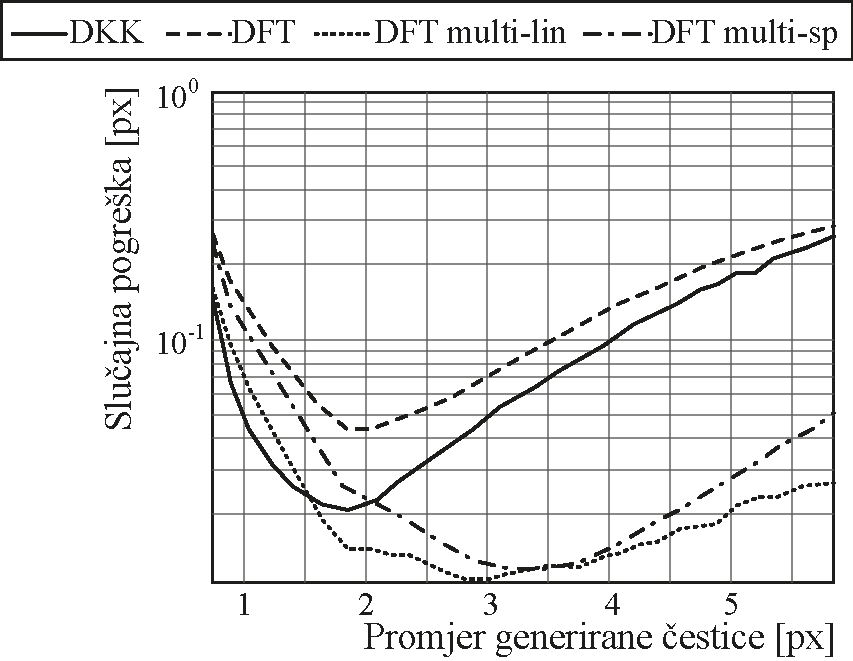
\includegraphics[width=10cm]{./4_PIVNesigurnost/slika4_7.pdf} 
		\caption{Efekt veličine promjera čestica na slučajnu pogrešku za prosječni pomak čestica od 3.5 pixela \cite{thielicke2014_article}}
		\label{sl:4.7}
	\end{figure}
	\item[Gustoća distribucije čestica] Kako su čestice nosioci informacije u PIV snimkama, gustoća njihove distribucije jako je bitna za dobru kvalitetu mjerenja. Vjerojatnost detekcije ispravnog pomaka znatno je veća ako je broj čestica unutar prozora ispitivanja oko 5. Broj uhvaćenih parova čestica u prozoru ispitivanja najviše ovisi o 3 faktora: gustoći čestica u snimci, količini pomaka koji se dogode unutar laserske ravnine, te količini pomaka izvan laserske ravnine (\textit{eng. out-of-plane motion}). 
	\item[Šum foto-senzora] Neželjeni šum na snimkama također smanjuje točnost mjerenja, a uzrokovan je ne-idealnom pretvorbom fotona električni signal na foto-senzoru. Jačina šuma ovisi o izvedbi senzora (CMOS ili CCD), te kvaliteti senzora. Analizu efekta šuma na točnost DPIV-a moguće je provjeriti dodavanjem umjetnog tzv. Gauss-ovog šuma (normalno distribuirani šum) u snimku. Ustanovljeno je kako obični DFT algoritam značajno gubi na točnosti zbog dodanog šum, dok DKK i DFT sa tehnikama deformacija prozora ispitivanja se mogu nositi sa šumom na snimkama.
	\item[Gubitak čestica unutar volumena ispitivanja (\textit{eng. out-of-plane motion})] U 2D DPIV analizi gubitak parova povezanih čestica je neizbježan zbog (uvijek) prisutnog 3D strujanja. Izgubljene čestice dovode do gubitka informacije, te samim time i povećane nesigurnosti zbog gubitka korelacijskog signala. Ovaj efekt moguće je simulirati na način da se umjetnim snimkama slučajno oduzme dio čestica na različitim pozicijama. U literaturi \cite{thielicke2014_phd} ustanovljeno je kako DFT algoritam ponovno dosta slabije reagira na gubitak čestica u odnosu na ostale.
	\item[Zamućenje pokreta] Uzrokovano je predugom ekspozicijom u kojoj dolazi do prebrzog kretanja čestica. Za vrijeme ekspozicije čestica se giba prevelikom brzinom te senzor kamere ne hvata trenutačno  njenu svjetlost, nego dobiva svjetlost čestice u više pozicija, zbog čega dolazi do zamućenja slike. Rješenje u vidu kraćeg trajanja ekspozicije, gdje se želi zamrznuti gibanje, često nije moguće zbog toga što onda premalo svjetlosti ulazi u senzor kamere. Zamućene slike iskrivljuju korelacijske vrhove, te tako povećavaju nesigurnost PIV analize. Efekt zamućenja slike, te koliku količinu nesigurnosti unosi u mjerenje može se simulirati tako da se umjetna slika konvoluira sa jednodimenzionalnim filtrom. DFT sa tehnikama deformacije prozora dosta su robusni, te su do određene mjere otporni i na ovaj utjecaj, dok obični DFT i DKK imaju povećanu nesigurnost.
	\item[Smicanje] U opisu tehnika deformacije prozora, predstavljen je otežavajući efekt smicanja unutar prozora ispitivanja. Opisana tehnika donekle limitira negativan utjecaj smicanja na točnost PIV analize. Smicanje se može simulirati primjenom kosog pomaka mreže snimke, te je u litraturi \cite{thielicke2014_phd} ustanovljeno kako obični DFT algoritam jako loše reagira na smicanje, DKK algoritam daje malo bolje rezultate, ali i dalje nedovoljno dobro kao algoritmi koji imaju uključene tehnike deformacije prozora, najveća točnost ostvarena je sa DFT algoritmom koji sadrži tehniku deformacije prozora, a koristi spline interpolaciju. 
\end{description}